\begin{figure}[htb]
\centering
\begin{tikzpicture}[scale = 10]
\tikzstyle{VertexStyle}=[shape = circle,	
								 minimum size = 1pt,
								 inner sep = 1.2pt,
                         draw]
\Vertex[x = 0.89000016450882, y = 0.730000019073486, L = \tiny {$x_1$}]{v0}
\Vertex[x = 0.410000026226044, y = 0.538000077009201, L = \tiny {$y_3$}]{v1}
\Vertex[x = 0.648000001907349, y = 0.631999969482422, L = \tiny {v}]{v2}
\Vertex[x = 0.409999966621399, y = 0.731999933719635, L = \tiny {$x_3$}]{v3}
\Vertex[x = 0.892000138759613, y = 0.537999987602234, L = \tiny {$y_1$}]{v4}
\Vertex[x = 0.198000028729439, y = 0.616000115871429, L = \tiny {$z$}]{v5}
\Edge[](v0)(v2)
\Edge[](v1)(v2)
\Edge[](v3)(v1)
\Edge[](v3)(v2)
\Edge[](v4)(v0)
\Edge[](v4)(v2)
\Edge[](v5)(v3)
\Edge[](v5)(v1)
\end{tikzpicture}
\caption{$K_2$ joined to this graph is $d_1$-choosable}
\label{fig:FinalContradiction}
\end{figure}
